\chapter{الدورة الخلوية والانقسام المتساوي}\label{ch:g11:cell-cycle-mitosis}

اهرس طرف جذر بصلة تحت غطاء زجاجي، ولوّنه، وانظر: بين مئات \omterm{def:g10:cells-common-unit:cell}{الخلايا}
الهادئة ذوات \omterm{def:g10:cells-common-unit:organelle}{النواة} المدورة، تبين قلة منها شيئًا آخر --- عصيات داكنة
على هيئة X مجتمعة في وسط \omterm{def:g10:cells-common-unit:cell}{الخلية}، أو طقمان من العصيات مشدودان متباعدين
نحو الطرفين، أو نواتان صغيرتان يتكون بينهما جدار. إنك تشاهد انقسام
\omterm{def:g10:cells-common-unit:cell}{الخلية} ملتقطًا في لحظات مختلفة، في نسيج ينمو مليمترًا في اليوم. وكل
انقسام من تلك الانقسامات يسلّم طقمين كاملين متطابقين من \omterm{def:g10:universal-dna:information}{الصبغيات} إلى
خليتين بنتين. ويتابع هذا الفصل \omterm{def:g10:cells-common-unit:cell}{خلية} عبر دورة كاملة، وينظر عن كثب في
الساعة التي تتوزع فيها \omterm{def:g10:universal-dna:information}{الصبغيات}.

\section{الدورة الخلوية}

\begin{definition}[الدورة الخلوية]\label{def:g11:cell-cycle-mitosis:cycle}
\emph{الدورة الخلوية}\index{دورة خلوية} هي تتابع الأحداث من ولادة
\omterm{def:g10:cells-common-unit:cell}{الخلية}، بالانقسام، إلى انقسامها هي إلى اثنتين. وتشمل \emph{الطور
البيني}، تنمو فيه \omterm{def:g10:cells-common-unit:cell}{الخلية} وتنسخ \omterm{def:g10:universal-dna:information}{DNA} فيها، و\emph{المرحلة M}، تنقسم
فيها \omterm{def:g10:cells-common-unit:organelle}{النواة} (\emph{الانقسام المتساوي}\index{انقسام متساوٍ}) ثم
\omterm{def:g10:cells-common-unit:cell}{السيتوبلازم} (\emph{انقسام \omterm{def:g10:cells-common-unit:cell}{السيتوبلازم}}). وللطور البيني ثلاثة أجزاء:
$\mathrm{G_1}$ (النمو)، وS (\omterm{def:g11:dna-replication:replication}{تضاعف DNA}،
\cref{ch:g11:dna-replication})، و$\mathrm{G_2}$ (التهيؤ للانقسام).
\end{definition}

\begin{omfigure}
\begin{tikzpicture}[font=\small]
  % pie: G1 11h, S 8h, G2 4h, M 1h  (24h) -> angles: G1 165°, S 120°, G2 60°, M 15°
  \fill[omDef!30] (0,0) -- (90:2.2) arc (90:-75:2.2) -- cycle;
  \fill[omProp!35] (0,0) -- (-75:2.2) arc (-75:-195:2.2) -- cycle;
  \fill[omMeth!35] (0,0) -- (-195:2.2) arc (-195:-255:2.2) -- cycle;
  \fill[omThm!50] (0,0) -- (-255:2.2) arc (-255:-270:2.2) -- cycle;
  \draw[thick] (0,0) circle (2.2);
  \foreach \a in {90,-75,-195,-255} \draw[thick] (0,0) -- (\a:2.2);
  \node at (10:1.3) {$\mathrm{G_1}$};
  \node at (-135:1.3) {S};
  \node at (-225:1.35) {$\mathrm{G_2}$};
  \node[anchor=south east] at (-262:2.35) {M};
  \node[anchor=west, align=left] at (2.6,1.3) {$\mathrm{G_1}$: نمو، نحو \qty{11}{h}};
  \node[anchor=west, align=left] at (2.6,0.5) {S: تضاعف DNA، \qty{8}{h}};
  \node[anchor=west, align=left] at (2.6,-0.3) {$\mathrm{G_2}$: تهيؤ، \qty{4}{h}};
  \node[anchor=west, align=left] at (2.6,-1.1) {M: انقسام متساوٍ وانقسام سيتوبلازم، \qty{1}{h}};
  \draw[->, thick] (100:2.5) arc (100:130:2.5);
\end{tikzpicture}

{\small \omterm{def:g11:cell-cycle-mitosis:cycle}{الدورة الخلوية} \omterm{def:g10:cells-common-unit:cell}{لخلية} بشرية منقسمة نموذجية، نحو 24 ساعة.
فالطور البيني ($\mathrm{G_1}$ وS و$\mathrm{G_2}$) يأخذ 23 منها؛
والانقسام نفسه ساعة واحدة. \omterm{def:g10:cells-common-unit:cell}{وخلايا} كثيرة تغادر الدورة بعد
$\mathrm{G_1}$ ولا تنقسم مرة أخرى أبدًا.}
\end{omfigure}

\begin{proposition}[DNA عبر الدورة]\label{prop:g11:cell-cycle-mitosis:dna}
سمِّ $q$ كمية \omterm{def:g10:universal-dna:information}{DNA} في \omterm{def:g10:cells-common-unit:organelle}{نواة} بعيد الانقسام. فهي تبقى عند $q$ خلال
$\mathrm{G_1}$، وترتفع باطراد إلى $2q$ أثناء S إذ تنسخ \omterm{def:g10:universal-dna:information}{الصبغيات}، وتبقى
عند $2q$ خلال $\mathrm{G_2}$ والجزء الأول من \omterm{def:g11:cell-cycle-mitosis:cycle}{الانقسام المتساوي}، وتعود
إلى $q$ في كل \omterm{def:g10:cells-common-unit:organelle}{نواة} بنت في نهاية الانقسام. وعدد \omterm{def:g10:universal-dna:information}{الصبغيات} لا يتغير أثناء
S: فكل \omterm{def:g10:universal-dna:information}{صبغي} ينسخ إلى \emph{\omterm{def:g11:cell-cycle-mitosis:chromosome}{صبغيدين}} متطابقين ممسكين معًا عند
\emph{قسيمهما المركزي}، ولا ينفصل إلى صبغيين إلا أثناء \omterm{def:g11:cell-cycle-mitosis:cycle}{الانقسام
المتساوي}.
\end{proposition}
\admitted

\begin{omfigure}
\begin{tikzpicture}
\begin{axis}[
  width=0.9\linewidth, height=5.4cm,
  axis x line=bottom, axis y line=left,
  xmin=0, xmax=50, ymin=0, ymax=2.8,
  xlabel={الزمن (h)}, ylabel={DNA في النواة},
  xlabel style={font=\small, at={(axis description cs:0.5,-0.1)}, anchor=north},
  ylabel style={font=\small},
  tick label style={font=\small}, xtick={0,11,19,23,24,35,43,47,48},
  xticklabels={0,11,19,23,,24,35,43,,48},
  ytick={1,2}, yticklabels={$q$, $2q$},
  clip=false,
]
\addplot[thick, omDef] coordinates {(0,1) (11,1) (19,2) (23,2) (23.9,2) (24,1) (35,1) (43,2) (47,2) (47.9,2) (48,1) (50,1)};
\node[font=\small, anchor=south] at (axis cs:5.5,2.25) {$\mathrm{G_1}$};
\node[font=\small, anchor=south] at (axis cs:15,2.25) {S};
\node[font=\small, anchor=south] at (axis cs:21,2.25) {$\mathrm{G_2}$};
\node[font=\small, anchor=south] at (axis cs:29.5,2.25) {$\mathrm{G_1}$};
\node[font=\small, anchor=south] at (axis cs:39,2.25) {S};
\node[font=\small, anchor=south] at (axis cs:45,2.25) {$\mathrm{G_2}$};
\node[font=\small, anchor=south, omThm] at (axis cs:23.5,2.55) {M};
\node[font=\small, anchor=south, omThm] at (axis cs:47.5,2.55) {M};
\draw[dashed, gray] (axis cs:11,0) -- (axis cs:11,2.2);
\draw[dashed, gray] (axis cs:19,0) -- (axis cs:19,2.2);
\draw[dashed, gray] (axis cs:23,0) -- (axis cs:23,2.2);
\draw[dashed, gray] (axis cs:24,0) -- (axis cs:24,2.2);
\draw[dashed, gray] (axis cs:35,0) -- (axis cs:35,2.2);
\draw[dashed, gray] (axis cs:43,0) -- (axis cs:43,2.2);
\draw[dashed, gray] (axis cs:47,0) -- (axis cs:47,2.2);
\end{axis}
\end{tikzpicture}

{\small كمية \omterm{def:g10:universal-dna:information}{DNA} في \omterm{def:g10:cells-common-unit:organelle}{نواة} واحدة على مدى دورتين متتاليتين من 24 ساعة.
فهي تتضاعف أثناء S وتنتصف في نهاية \omterm{def:g11:cell-cycle-mitosis:cycle}{الانقسام المتساوي}؛ \omterm{def:g10:cells-common-unit:cell}{والخلية} البنت
تبدأ دائمًا بالكمية $q$.}
\end{omfigure}

\begin{example}[قراءة المنحني]\label{ex:g11:cell-cycle-mitosis:reading}
\omterm{def:g10:cells-common-unit:cell}{الخلية} التي تقاس عند $2q$ قد تكون في $\mathrm{G_2}$ أو في أول \omterm{def:g11:cell-cycle-mitosis:cycle}{الانقسام
المتساوي}؛ وعند $1.5q$ هي في S قطعًا، في منتصف التضاعف؛ وعند $q$ هي في
$\mathrm{G_1}$ --- أو قد غادرت الدورة إلى الأبد، كالعصبون أو الليف
العضلي، وهما يبقيان عند $q$ مدى الحياة. والنسيج الذي كل \omterm{def:g10:cells-common-unit:cell}{خلية} فيه عند
$q$ نسيج كف عن الانقسام.
\end{example}

\section{الصبغيات مرئيةً}

\begin{definition}[الصبغي والصبغيد والنمط الصبغي]\label{def:g11:cell-cycle-mitosis:chromosome}
\emph{\omterm{def:g10:universal-dna:information}{الصبغي}} جزيء \omterm{def:g10:universal-dna:information}{DNA} واحد مع بروتيناته الحازمة. وهو بين الانقسامات
خيط منشور غير مرئي؛ وفي بداية \omterm{def:g11:cell-cycle-mitosis:cycle}{الانقسام المتساوي} يتكوّر في عصية مكتنزة
ترى تحت المجهر الضوئي. وبعد التضاعف يتألف كل \omterm{def:g10:universal-dna:information}{صبغي} من
\emph{صبغيدين}\index{صبغيد} متطابقين، ملتحمين عند \emph{القسيم
المركزي}\index{قسيم مركزي}: وهو شكل X المألوف. و\emph{النمط
الصبغي}\index{نمط صبغي} \omterm{def:g10:biodiversity-scales:species}{لنوع} ما هو طقم صبغياته الكامل، مصوَّرًا في
الطور الاستوائي ومرتَّبًا أزواجًا بحسب الحجم: فللخلية البشرية 46
صبغيًا، في 23 زوجًا، وعضوا الزوج \emph{متماثلان} --- \omterm{def:g10:universal-dna:gene}{المورّثات} نفسها
في المواضع نفسها، واحد من كل والد.
\end{definition}

\begin{omfigure}
\begin{tikzpicture}[font=\scriptsize, line cap=round]
  % 22 autosome pairs of decreasing size, then X and Y; each chromosome = two chromatids
  \tikzset{chrom/.style={line width=2.6pt, omDef!75}}
  \foreach \n/\h/\c in {1/2.4/0.55, 2/2.3/0.5, 3/2.0/0.5, 4/1.9/0.35, 5/1.8/0.35, 6/1.7/0.45, 7/1.55/0.42, 8/1.45/0.4}
    { \pgfmathsetmacro{\x}{(\n-1)*1.55}
      \draw[chrom] (\x,0) -- (\x,\h); \draw[chrom] (\x+0.22,0) -- (\x+0.22,\h);
      \fill[omThm] (\x+0.11,{\h*\c}) circle (2pt);
      \node[anchor=north] at (\x+0.11,-0.08) {\n}; }
  \foreach \n/\h/\c in {9/1.4/0.35, 10/1.35/0.35, 11/1.35/0.4, 12/1.3/0.3, 13/1.1/0.15, 14/1.05/0.15, 15/1.0/0.15, 16/0.9/0.45}
    { \pgfmathsetmacro{\x}{(\n-9)*1.55}
      \draw[chrom] (\x,-3.2) -- (\x,-3.2+\h); \draw[chrom] (\x+0.22,-3.2) -- (\x+0.22,-3.2+\h);
      \fill[omThm] (\x+0.11,{-3.2+\h*\c}) circle (2pt);
      \node[anchor=north] at (\x+0.11,-3.28) {\n}; }
  \foreach \n/\h/\c in {17/0.85/0.3, 18/0.8/0.2, 19/0.65/0.5, 20/0.65/0.5, 21/0.5/0.2, 22/0.5/0.2}
    { \pgfmathsetmacro{\x}{(\n-17)*1.55}
      \draw[chrom] (\x,-5.6) -- (\x,-5.6+\h); \draw[chrom] (\x+0.22,-5.6) -- (\x+0.22,-5.6+\h);
      \fill[omThm] (\x+0.11,{-5.6+\h*\c}) circle (2pt);
      \node[anchor=north] at (\x+0.11,-5.68) {\n}; }
  % sex chromosomes
  \draw[chrom] (9.3,-5.6) -- (9.3,-4.1); \draw[chrom] (9.52,-5.6) -- (9.52,-4.1); \fill[omThm] (9.41,-4.85) circle (2pt);
  \node[anchor=north] at (9.41,-5.68) {X};
  \draw[chrom] (10.85,-5.6) -- (10.85,-5.1); \draw[chrom] (11.07,-5.6) -- (11.07,-5.1); \fill[omThm] (10.96,-5.5) circle (2pt);
  \node[anchor=north] at (10.96,-5.68) {Y};
\end{tikzpicture}

{\small \omterm{def:g11:cell-cycle-mitosis:chromosome}{نمط صبغي} بشري، تخطيطيًا: أزواج \omterm{def:g10:universal-dna:information}{الصبغيات} العادية الاثنان
والعشرون مرقمة بترتيب الحجم المتناقص، ثم الصبغيان الجنسيان --- X وY
هنا، فهو ذكر. وكل \omterm{def:g10:universal-dna:information}{صبغي} مرسوم بصبغيديه، \omterm{def:g11:cell-cycle-mitosis:chromosome}{والقسيم المركزي} بالأحمر.}
\end{omfigure}

\begin{omfigure}
\begin{tikzpicture}[font=\small, line cap=round]
  % single chromatid chromosome
  \draw[line width=5pt, omDef!70] (0,-1.2) -- (0,1.2);
  \fill[omThm] (0,0.2) circle (3.5pt);
  \node[anchor=north, align=center] at (0,-1.5) {قبل المرحلة S:\\ صبغيد واحد};
  % arrow
  \draw[->, thick] (1.2,0) -- (2.6,0) node[midway, above] {S};
  % two chromatid chromosome
  \draw[line width=5pt, omDef!70] (3.6,-1.2) .. controls (3.75,-0.3) and (3.75,0.3) .. (3.6,1.2);
  \draw[line width=5pt, omDef!70] (4.2,-1.2) .. controls (4.05,-0.3) and (4.05,0.3) .. (4.2,1.2);
  \fill[omThm] (3.9,0.2) circle (3.5pt);
  \node[anchor=north, align=center] at (3.9,-1.5) {بعد المرحلة S:\\ صبغيدان متطابقان};
  \draw[->] (5.6,0.2) -- (4.15,0.2) node[pos=0, anchor=west] {القسيم المركزي};
  \draw[->] (5.6,0.9) -- (4.35,0.9) node[pos=0, anchor=west] {صبغيد};
  % after anaphase
  \draw[->, thick] (8.6,0) -- (10.0,0) node[midway, above] {الطور الانفصالي};
  \draw[line width=5pt, omDef!70] (10.8,-1.2) -- (10.8,1.2);
  \fill[omThm] (10.8,0.2) circle (3.5pt);
  \draw[line width=5pt, omDef!70] (11.8,-1.2) -- (11.8,1.2);
  \fill[omThm] (11.8,0.2) circle (3.5pt);
  \node[anchor=north, align=center] at (11.3,-1.5) {صبغيان،\\ واحد لكل خلية};
\end{tikzpicture}

{\small \omterm{def:g10:universal-dna:information}{صبغي} واحد عبر الدورة. التضاعف يحوله إلى \omterm{def:g11:cell-cycle-mitosis:chromosome}{صبغيدين} ملتحمين عند
\omterm{def:g11:cell-cycle-mitosis:chromosome}{القسيم المركزي}؛ والطور الانفصالي يفصلهما إلى صبغيين أحاديي \omterm{def:g11:cell-cycle-mitosis:chromosome}{الصبغيد}،
واحد لكل \omterm{def:g10:cells-common-unit:cell}{خلية} بنت. وعدد \omterm{def:g10:universal-dna:information}{الصبغيات} لا يتغير إلا في الطور الانفصالي.}
\end{omfigure}

\section{الانقسام المتساوي، خطوة خطوة}

\begin{proposition}[أطوار الانقسام المتساوي الأربعة]\label{prop:g11:cell-cycle-mitosis:stages}
\omterm{def:g11:cell-cycle-mitosis:cycle}{الانقسام المتساوي} حركة متصلة، توصف في أربعة أطوار.
\begin{enumerate}
  \item \emph{الطور التمهيدي}: تتكثف \omterm{def:g10:universal-dna:information}{الصبغيات} في عصيات مرئية ثنائية
        \omterm{def:g11:cell-cycle-mitosis:chromosome}{الصبغيد}؛ وينهار الغلاف النووي؛ ويتكون \emph{مغزل} من ألياف
        بروتينية بين قطبي \omterm{def:g10:cells-common-unit:cell}{الخلية}.
  \item \emph{الطور الاستوائي}: تصطف \omterm{def:g10:universal-dna:information}{الصبغيات}، وهي متصلة بألياف
        المغزل بقسيماتها المركزية، على المستوي الاستوائي \omterm{def:g10:cells-common-unit:cell}{للخلية}.
  \item \emph{الطور الانفصالي}: تنشطر القسيمات المركزية؛ ويشد صبغيدا
        كل \omterm{def:g10:universal-dna:information}{صبغي}، وقد صارا صبغيين، إلى قطبين متقابلين بالألياف
        المتقصرة.
  \item \emph{الطور النهائي}: يتكون غلاف نووي من جديد حول كل طقم؛
        وتنشر \omterm{def:g10:universal-dna:information}{الصبغيات}. ثم يقسم انقسام \omterm{def:g10:cells-common-unit:cell}{السيتوبلازم} السيتوبلازمَ ---
        بالانخماص في \omterm{def:g10:cells-common-unit:cell}{الخلايا} الحيوانية، وببناء جدار جديد في \omterm{def:g10:cells-common-unit:cell}{الخلايا}
        النباتية.
\end{enumerate}
وتتلقى كل \omterm{def:g10:cells-common-unit:cell}{خلية} بنت صبغيدًا واحدًا من كل \omterm{def:g10:universal-dna:information}{صبغي}: أي عدد \omterm{def:g10:universal-dna:information}{الصبغيات} نفسه
الذي عند الأم، حاملًا \omterm{def:g10:universal-dna:information}{DNA} نفسه.
\end{proposition}
\admitted

\begin{omfigure}
\begin{tikzpicture}[font=\small, line cap=round]
  \tikzset{cellb/.style={draw, thick, fill=omDef!5, rounded corners=10pt, minimum width=2.9cm, minimum height=2.6cm},
           chr/.style={line width=3pt, omDef!80}, cen/.style={fill=omThm}}
  % prophase
  \begin{scope}
    \node[cellb] at (0,0) {};
    \draw[thick, dashed, gray] (0,0) circle (0.95);
    \draw[chr] (-0.5,0.5) .. controls (-0.35,0.1) .. (-0.5,-0.3); \draw[chr] (-0.2,0.5) .. controls (-0.35,0.1) .. (-0.2,-0.3); \fill[cen] (-0.35,0.1) circle (2pt);
    \draw[chr] (0.2,0.6) .. controls (0.35,0.2) .. (0.2,-0.2); \draw[chr] (0.5,0.6) .. controls (0.35,0.2) .. (0.5,-0.2); \fill[cen] (0.35,0.2) circle (2pt);
    \node[anchor=north, align=center] at (0,-1.45) {الطور التمهيدي};
  \end{scope}
  % metaphase
  \begin{scope}[xshift=3.6cm]
    \node[cellb] at (0,0) {};
    \fill (0,1.1) circle (2pt); \fill (0,-1.1) circle (2pt);
    \foreach \x in {-0.45,0.45} { \draw[gray] (0,1.1) -- (\x,0.05); \draw[gray] (0,-1.1) -- (\x,-0.05); }
    \foreach \x in {-0.45,0.45} {
      \draw[chr] (\x-0.13,0.55) .. controls (\x,0.0) .. (\x-0.13,-0.55);
      \draw[chr] (\x+0.13,0.55) .. controls (\x,0.0) .. (\x+0.13,-0.55);
      \fill[cen] (\x,0) circle (2pt);
    }
    \draw[dashed, gray] (-1.3,0) -- (1.3,0);
    \node[anchor=north, align=center] at (0,-1.45) {الطور الاستوائي};
  \end{scope}
  % anaphase
  \begin{scope}[xshift=7.2cm]
    \node[cellb] at (0,0) {};
    \fill (0,1.1) circle (2pt); \fill (0,-1.1) circle (2pt);
    \foreach \x in {-0.45,0.45} { \draw[gray] (0,1.1) -- (\x,0.6); \draw[gray] (0,-1.1) -- (\x,-0.6); }
    \foreach \x in {-0.45,0.45} {
      \draw[chr] (\x,0.6) .. controls (\x-0.1,0.4) .. (\x-0.25,0.05);
      \draw[chr] (\x,0.6) .. controls (\x+0.1,0.4) .. (\x+0.25,0.05);
      \fill[cen] (\x,0.6) circle (2pt);
      \draw[chr] (\x,-0.6) .. controls (\x-0.1,-0.4) .. (\x-0.25,-0.05);
      \draw[chr] (\x,-0.6) .. controls (\x+0.1,-0.4) .. (\x+0.25,-0.05);
      \fill[cen] (\x,-0.6) circle (2pt);
    }
    \node[anchor=north, align=center] at (0,-1.45) {الطور الانفصالي};
  \end{scope}
  % telophase
  \begin{scope}[xshift=10.8cm]
    \draw[thick, fill=omDef!5] (-1.45,1.3) .. controls (-1.6,0.3) and (-0.3,0.3) .. (0,0) .. controls (-0.3,-0.3) and (-1.6,-0.3) .. (-1.45,-1.3) -- cycle;
    \draw[thick, fill=omDef!5] (1.45,1.3) .. controls (1.6,0.3) and (0.3,0.3) .. (0,0) .. controls (0.3,-0.3) and (1.6,-0.3) .. (1.45,-1.3) -- cycle;
    \draw[thick, fill=omDef!5, rounded corners=10pt] (-1.45,-1.3) rectangle (1.45,1.3);
    \draw[thick, fill=white] (-1.45,1.3) .. controls (-1.6,0.3) and (-0.3,0.3) .. (0,0) .. controls (-0.3,-0.3) and (-1.6,-0.3) .. (-1.45,-1.3);
    \draw[thick, fill=white] (1.45,1.3) .. controls (1.6,0.3) and (0.3,0.3) .. (0,0) .. controls (0.3,-0.3) and (1.6,-0.3) .. (1.45,-1.3);
    \draw[thick, dashed, gray] (-0.75,0) circle (0.5); \draw[thick, dashed, gray] (0.75,0) circle (0.5);
    \foreach \x in {-0.9,-0.6,0.6,0.9} \draw[chr] (\x,0.25) -- (\x,-0.25);
    \node[anchor=north, align=center] at (0,-1.45) {الطور النهائي\\ وانقسام السيتوبلازم};
  \end{scope}
\end{tikzpicture}

{\small \omterm{def:g11:cell-cycle-mitosis:cycle}{انقسام متساوٍ} \omterm{def:g10:cells-common-unit:cell}{لخلية} فيها صبغيان ($2n = 2$)، كل منهما مؤلف من
\omterm{def:g11:cell-cycle-mitosis:chromosome}{صبغيدين} من قبل. الطور التمهيدي: تكثف، وغلاف زال. والطور الاستوائي:
اصطفاف على الاستواء، وقسيمات مركزية متصلة بالمغزل. والطور الانفصالي:
\omterm{def:g11:cell-cycle-mitosis:chromosome}{صبغيدان} يشدان متباعدين إلى القطبين. والطور النهائي: نواتان تتكونان من
جديد وتنقسم \omterm{def:g10:cells-common-unit:cell}{الخلية}.}
\end{omfigure}

\begin{omfigure}
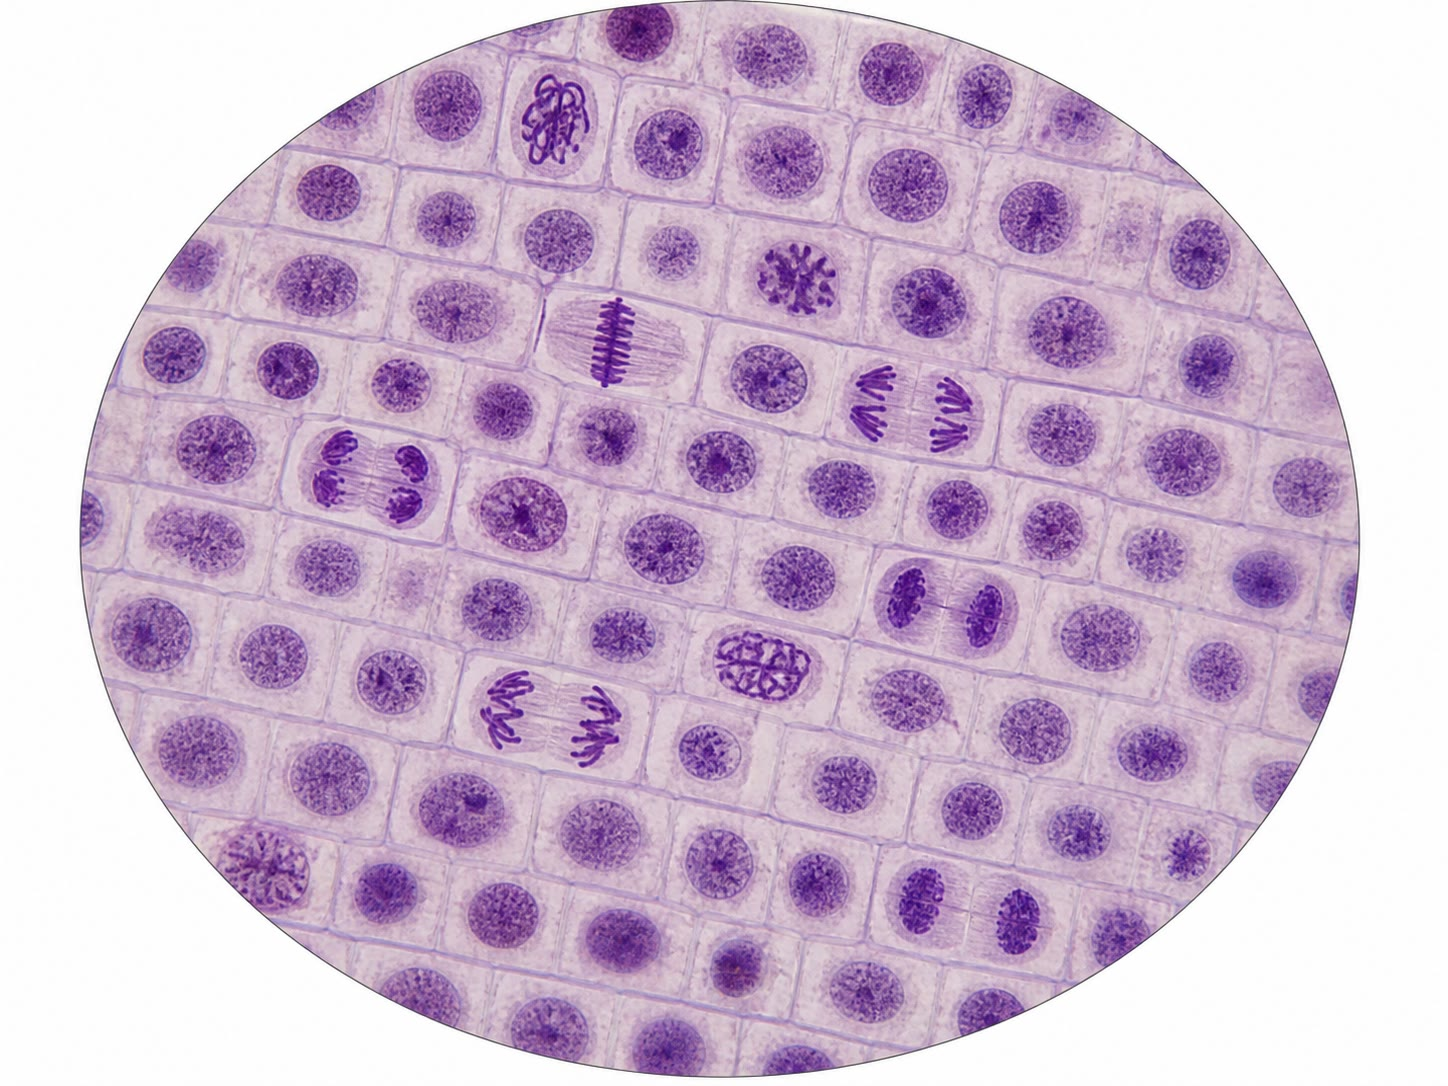
\includegraphics[width=0.58\linewidth]{images/book2/ai/g11-mitosis-root-tip.jpg}

{\small هرس طرف جذر بصلة تحت المجهر الضوئي. معظم \omterm{def:g10:cells-common-unit:cell}{الخلايا} في الطور
البيني؛ وقلة منها تبين صبغيات متكثفة في أطوار مختلفة من \omterm{def:g11:cell-cycle-mitosis:cycle}{الانقسام
المتساوي}. وعدّ نسبة \omterm{def:g10:cells-common-unit:cell}{الخلايا} في كل طور يقيس كم يدوم كل طور.}
\end{omfigure}

\begin{example}[العدّ في طرف الجذر]\label{ex:g11:cell-cycle-mitosis:count}
من بين 600 \omterm{def:g10:cells-common-unit:cell}{خلية} عدّت في طرف جذر، 540 في الطور البيني و60 في \omterm{def:g11:cell-cycle-mitosis:cycle}{الانقسام
المتساوي}: أي \emph{دليل انقسامي} قدره 10\%. فإذا دامت الدورة 20 ساعة،
دام الانقسام نحو $0.10 \times 20 = \qty{2}{h}$؛ وإذا كانت 36 من
\omterm{def:g10:cells-common-unit:cell}{الخلايا} المنقسمة الستين في الطور التمهيدي، أخذ الطور التمهيدي $36/60$
من تينك الساعتين، أي نحو 72 دقيقة، بينما يأخذ الطور الانفصالي، وقد
رئي في 4 \omterm{def:g10:cells-common-unit:cell}{خلايا} فقط، نحو 8 دقائق. فأندر الأطوار أسرعها.
\end{example}

\begin{method}[عدّ الصبغيات والصبغيدات]\label{met:g11:cell-cycle-mitosis:counting}
\omterm{def:g10:biodiversity-scales:species}{لنوع} فيه $2n$ صبغيًا:
\begin{enumerate}
  \item في $\mathrm{G_1}$: $2n$ صبغيًا، لكل منها \omterm{def:g11:cell-cycle-mitosis:chromosome}{صبغيد} واحد، \omterm{def:g10:universal-dna:information}{وDNA}
        قدره $q$؛
  \item بعد S، وخلال $\mathrm{G_2}$ والطورين التمهيدي والاستوائي:
        $2n$ صبغيًا، لكل منها \omterm{def:g11:cell-cycle-mitosis:chromosome}{صبغيدان} ($4n$ صبغيدًا)، \omterm{def:g10:universal-dna:information}{وDNA} قدره $2q$؛
  \item من الطور الانفصالي: $4n$ صبغيًا أحادي \omterm{def:g11:cell-cycle-mitosis:chromosome}{الصبغيد} في \omterm{def:g10:cells-common-unit:cell}{الخلية}،
        و$2n$ متجهًا إلى كل قطب؛
  \item في كل \omterm{def:g10:cells-common-unit:cell}{خلية} بنت: $2n$ صبغيًا، لكل منها \omterm{def:g11:cell-cycle-mitosis:chromosome}{صبغيد} واحد، \omterm{def:g10:universal-dna:information}{وDNA} قدره
        $q$.
\end{enumerate}
ويصير \omterm{def:g11:cell-cycle-mitosis:chromosome}{الصبغيد} صبغيًا لحظة انشطار قسيمه المركزي.
\end{method}

\begin{example}[أرقام بشرية]\label{ex:g11:cell-cycle-mitosis:human}
\omterm{def:g10:cells-common-unit:cell}{الخلية} البشرية في الطور الاستوائي تحمل 46 صبغيًا و92 صبغيدًا؛ وفي
الطور الانفصالي، 92 صبغيًا، منها 46 يتجه إلى كل قطب؛ وكل بنت، 46
صبغيًا لكل منها \omterm{def:g11:cell-cycle-mitosis:chromosome}{صبغيد} واحد، تحوي \omterm{def:g10:universal-dna:information}{DNA} نفسه الذي كان عند الأم في بداية
دورتها بالضبط.
\end{example}

\section{ما فائدة الانقسام المتساوي}

\begin{proposition}[التطابق واستعمالاته]\label{prop:g11:cell-cycle-mitosis:conformity}
لما كان التضاعف أمينًا \omterm{def:g11:cell-cycle-mitosis:cycle}{والانقسام المتساوي} يوزع \omterm{def:g11:cell-cycle-mitosis:chromosome}{الصبغيدات} توزيعًا
دقيقًا، حملت كل \omterm{def:g10:cells-common-unit:cell}{خلية} من جسم عديد \omterm{def:g10:cells-common-unit:cell}{الخلايا} \omterm{def:g10:universal-dna:information}{المعلومة الوراثية} نفسها التي
في البيضة الملقحة التي انحدرت منها. \omterm{def:g11:cell-cycle-mitosis:cycle}{والانقسام المتساوي} هو آلية النمو
(الجنين، طرف الجذر)، والتجديد (الجلد، وبطانة المعي، والدم: فنقي العظم
وحده يصنع نحو $\num{2e11}$ \omterm{def:g10:cells-common-unit:cell}{خلية} في اليوم)، والإصلاح (التئام الجروح)؛
وهو في حقيقيات \omterm{def:g10:cells-common-unit:organelle}{النواة} الوحيدة \omterm{def:g10:cells-common-unit:cell}{الخلية} التكاثر نفسه. أما ضبطه --- قرار
دخول الدورة، والتحققات قبل S وقبل الطور الانفصالي --- فموضوع
\cref{ch:g11:cancer}.
\end{proposition}
\admitted

\begin{remark}[ليس كل شيء ينقسم]\label{rem:g11:cell-cycle-mitosis:notall}
معظم العصبونات \omterm{def:g10:cells-common-unit:cell}{وخلايا} عضلة القلب تغادر الدورة في الطفولة الباكرة ولا
تعود إليها أبدًا: فالأذى الذي يصيبها لا يصلحه انقسام، ولذلك تخلف إصابة
النخاع الشوكي أو نوبة قلبية خسارة دائمة. أما \omterm{def:g10:cells-common-unit:cell}{خلايا} الكبد فترتاح في
$\mathrm{G_1}$ أشهرًا لكنها تعود إلى الدورة حين يستأصل جزء من الكبد،
فتنمّي العضو من جديد في غضون أسابيع. وأي \omterm{def:g10:cells-common-unit:cell}{الخلايا} يجوز أن تنقسم، ومتى،
من أشد ما ينظَّم في الجسم.
\end{remark}

\section{تمارين}

\begin{exercise}[$\star$]\label{exo:g11:cell-cycle-mitosis:1}
سمِّ مراحل \omterm{def:g11:cell-cycle-mitosis:cycle}{الدورة الخلوية} الأربع وقل ماذا يحدث في كل منها.
\end{exercise}

\begin{exercise}[$\star$]\label{exo:g11:cell-cycle-mitosis:2}
عرّف \omterm{def:g11:cell-cycle-mitosis:chromosome}{الصبغيد} \omterm{def:g11:cell-cycle-mitosis:chromosome}{والقسيم المركزي}. ومتى يكون \omterm{def:g10:universal-dna:information}{للصبغي} \omterm{def:g11:cell-cycle-mitosis:chromosome}{صبغيدان}؟
\end{exercise}

\begin{exercise}[$\star$]\label{exo:g11:cell-cycle-mitosis:3}
اسرد أطوار \omterm{def:g11:cell-cycle-mitosis:cycle}{الانقسام المتساوي} الأربعة بحدث رئيسي واحد لكل منها.
\end{exercise}

\begin{exercise}[$\star$]\label{exo:g11:cell-cycle-mitosis:4}
\omterm{def:g10:cells-common-unit:organelle}{نواة} فيها $1.5q$ من \omterm{def:g10:universal-dna:information}{DNA}. ففي أي مرحلة \omterm{def:g10:cells-common-unit:cell}{الخلية}؟
\end{exercise}

\begin{exercise}[$\star$]\label{exo:g11:cell-cycle-mitosis:5}
كم صبغيًا وكم صبغيدًا في \omterm{def:g10:cells-common-unit:cell}{خلية} بشرية في $\mathrm{G_2}$؟
\end{exercise}

\begin{exercise}[$\star\star$]\label{exo:g11:cell-cycle-mitosis:6}
من شكل كمية \omterm{def:g10:universal-dna:information}{DNA}، أعطِ مدة كل مرحلة وقل في أي المراحل توجد \omterm{def:g10:cells-common-unit:cell}{خلية} عند
$2q$.
\end{exercise}

\begin{exercise}[$\star\star$]\label{exo:g11:cell-cycle-mitosis:7}
لفأر $2n = 40$. أعطِ عدد \omterm{def:g10:universal-dna:information}{الصبغيات} وعدد \omterm{def:g11:cell-cycle-mitosis:chromosome}{الصبغيدات} في \omterm{def:g10:cells-common-unit:cell}{خلية} في الطور
الاستوائي، وفي الطور الانفصالي (\omterm{def:g10:cells-common-unit:cell}{الخلية} كلها)، وفي \omterm{def:g10:cells-common-unit:cell}{خلية} بنت.
\end{exercise}

\begin{exercise}[$\star\star$]\label{exo:g11:cell-cycle-mitosis:8}
في طرف جذر، عدّت 800 \omterm{def:g10:cells-common-unit:cell}{خلية}: 720 في الطور البيني، و48 في التمهيدي، و16
في الاستوائي، و6 في الانفصالي، و10 في النهائي. احسب الدليل الانقسامي،
ولدورة من 24 ساعة، مدة كل طور.
\end{exercise}

\begin{exercise}[$\star\star$]\label{exo:g11:cell-cycle-mitosis:9}
الكولشيسين، وهو دواء يستخلص من زعفران الخريف، يمنع تكوّن المغزل. تنبأ
بما يحدث \omterm{def:g10:cells-common-unit:cell}{لخلية} منقسمة تعالج به، ولماذا يستعمله البيولوجيون لتحضير
الأنماط الصبغية.
\end{exercise}

\begin{exercise}[$\star\star$]\label{exo:g11:cell-cycle-mitosis:10}
فسّر لماذا يجب أن تتكثف \omterm{def:g10:universal-dna:information}{الصبغيات} قبل أن تحرَّك، ولماذا تنشر من جديد
بعد ذلك.
\end{exercise}

\begin{exercise}[$\star\star$]\label{exo:g11:cell-cycle-mitosis:11}
بيضة ملقحة تنقسم كل 12 ساعة في الأيام الأولى. فكم \omterm{def:g10:cells-common-unit:cell}{خلية} بعد 5 أيام؟
وهل يحتاج كل انقسام إلى $\mathrm{G_1}$ كاملة؟
\end{exercise}

\begin{exercise}[$\star\star\star$]\label{exo:g11:cell-cycle-mitosis:12}
في الطور الانفصالي يخفق صبغيدا \omterm{def:g10:universal-dna:information}{صبغي} واحد في الانفصال ويذهبان معًا إلى
القطب نفسه. صف الخليتين البنتين (عدد \omterm{def:g10:universal-dna:information}{الصبغيات}، \omterm{def:g10:universal-dna:information}{وDNA}) وفسّر لماذا يكون
مثل هذا الخطأ، في \omterm{def:g10:cells-common-unit:cell}{خلية} جسدية، بلا أثر عادةً لكنه خطر في بعض الحالات.
\end{exercise}

\begin{exercise}[$\star\star\star$]\label{exo:g11:cell-cycle-mitosis:13}
ينتج نقي العظم $\num{2e11}$ \omterm{def:g10:cells-common-unit:cell}{خلية} دم في اليوم. فإذا دارت \omterm{def:g10:cells-common-unit:cell}{خلية} سلف في
النقي دورتها في 24 ساعة، فقدّر كم سلفًا ينقسم في أي لحظة، وعلّق على ما
يفعله دواء يحصر \omterm{def:g11:cell-cycle-mitosis:cycle}{الانقسام المتساوي} بالدم في غضون أسبوع.
\end{exercise}

\begin{exercise}[$\star\star\star$]\label{exo:g11:cell-cycle-mitosis:14}
فسّر لماذا يحضَّر \omterm{def:g11:cell-cycle-mitosis:chromosome}{النمط الصبغي} من \omterm{def:g10:cells-common-unit:cell}{خلايا} موقوفة في الطور الاستوائي لا
في الطور البيني ولا الانفصالي.
\end{exercise}

\begin{exercise}[$\star\star\star$]\label{exo:g11:cell-cycle-mitosis:15}
استؤصل ثلثا كبد؛ وفي غضون ثلاثة أسابيع نما من جديد. باستعمال \omterm{def:g11:cell-cycle-mitosis:cycle}{الدورة
الخلوية}، صف ما فعلته خلاياه، وقل كيف كان محتوى \omterm{def:g10:cells-common-unit:cell}{خلايا} الكبد من \omterm{def:g10:universal-dna:information}{DNA} في
اليوم الثالث قياسًا إلى اليوم صفر.
\end{exercise}

\section{مسألة: جدول أوقات طرف الجذر}

\begin{problem}[{مسألة نهاية الأسبوع --- طرف جذر يعد خلية خلية: مدة
كل طور من الدورة، وDNA في كل لحظة، والخلايا التي يصنعها جذر في يوم،
ودقائق الطور الانفصالي الثماني}]
\label{pb:g11:cell-cycle-mitosis:1}
يهرس صف طرف جذر ثوم ($2n = 16$) ويلونه ويعد 1000 \omterm{def:g10:cells-common-unit:cell}{خلية} في منطقة النمو:
900 في الطور البيني، و60 في التمهيدي، و18 في الاستوائي، و8 في
الانفصالي، و14 في النهائي. وتعطي قياسات مستقلة دورة هذه \omterm{def:g10:cells-common-unit:cell}{الخلايا} 20
ساعة. وخذ منطقة النمو محتوية على 20\,000 \omterm{def:g10:cells-common-unit:cell}{خلية}.

\medskip
\noindent\textbf{الجزء الأول --- الدليل الانقسامي.}
\begin{enumerate}
  \item احسب الدليل الانقسامي للنسيج.
  \item بافتراض أن نسبة \omterm{def:g10:cells-common-unit:cell}{الخلايا} في طور ما تساوي نسبة الدورة التي تقضى
        فيه، احسب مدة \omterm{def:g11:cell-cycle-mitosis:cycle}{الانقسام المتساوي}.
  \item احسب مدة كل من الأطوار الأربعة.
  \item أي طور هو الأقصر؟ اقترح لماذا يستطيع أن يكون بهذه السرعة.
  \item لماذا تقتضي الطريقة عدّ \omterm{def:g10:cells-common-unit:cell}{خلايا} كثيرة، ولماذا يجب أن تكون من
        منطقة النمو وحدها؟
\end{enumerate}

\medskip
\noindent\textbf{الجزء الثاني --- \omterm{def:g10:universal-dna:information}{الصبغيات} \omterm{def:g10:universal-dna:information}{وDNA}.}
\begin{enumerate}[resume]
  \item كم صبغيًا وكم صبغيدًا تحمل \omterm{def:g10:cells-common-unit:cell}{خلية} ثوم في الطور الاستوائي؟
  \item كم صبغيًا يتحرك في \omterm{def:g10:cells-common-unit:cell}{خلية} في الطور الانفصالي، وكم يبلغ كل قطب؟
  \item إذا سميت $q$ كمية \omterm{def:g10:universal-dna:information}{DNA} في \omterm{def:g10:cells-common-unit:cell}{خلية} بنت، فأعطِ محتوى \omterm{def:g10:universal-dna:information}{DNA} في \omterm{def:g10:cells-common-unit:cell}{خلية} في
        الطور التمهيدي، وفي الانفصالي (\omterm{def:g10:cells-common-unit:cell}{الخلية} كلها)، وفي النهائي (كل
        \omterm{def:g10:cells-common-unit:organelle}{نواة}).
  \item من \omterm{def:g10:cells-common-unit:cell}{الخلايا} التسعمئة في الطور البيني، كم منها تقريبًا في S، إذا
        أخذت $\mathrm{G_1}$ وS و$\mathrm{G_2}$ 8 و7 و4 ساعات؟
  \item يجد تلميذ \omterm{def:g10:cells-common-unit:cell}{خلية} فيها 32 صبغيًا أحادي \omterm{def:g11:cell-cycle-mitosis:chromosome}{الصبغيد} منتشرة في
        \omterm{def:g10:cells-common-unit:cell}{السيتوبلازم}. فأي طور هو، وما الذي حدث للتو؟
\end{enumerate}

\medskip
\noindent\textbf{الجزء الثالث --- إنتاج الجذر.}
\begin{enumerate}[resume]
  \item إذا دارت كل \omterm{def:g10:cells-common-unit:cell}{خلية} من منطقة النمو دورتها في 20 ساعة، فكم \omterm{def:g10:cells-common-unit:cell}{خلية}
        جديدة تنتج المنطقة في الساعة؟
  \item كل \omterm{def:g10:cells-common-unit:cell}{خلية} جديدة، متى خرجت من منطقة النمو، تستطيل إلى نحو
        \qty{100}{\micro m}. ففي صف من \omterm{def:g10:cells-common-unit:cell}{الخلايا} عرضه \omterm{def:g10:cells-common-unit:cell}{خلية} واحدة، بكم
        يطول الجذر في اليوم؟ قارن بالمليمتر \qty{1}{mm} المشاهد في
        اليوم وفسّر الفرق.
  \item على كل \omterm{def:g10:cells-common-unit:cell}{خلية} بنت أن تنسخ $2n = 16$ صبغيًا، أي نحو
        $\num{1.6e10}$ زوج قواعد إجمالًا. فبشوكات تضيف 50 نوكليوتيدًا
        في الثانية، كم منشأً يلزم لإتمام ذلك في ساعات S السبع؟
  \item يوضع الجذر في البرد (\qty{4}{\celsius}) يومًا. تنبأ بالتغير في
        الأعداد، وفي الدليل الانقسامي إذا أبطأ البرد الأطوار كلها
        بالقدر نفسه.
  \item مبيد أعشاب يحصر \omterm{prop:g11:dna-replication:forks}{بوليميراز DNA}. فبعد يوم، أي الأطوار يظل يرى في
        الهرسة، وأيها يكون قد اختفى؟ فسّر.
\end{enumerate}

\medskip
\noindent\textbf{الجزء الرابع --- حكم الأعداد.}
\begin{enumerate}[resume]
  \item يعد صف ثانٍ النسيج نفسه فيجد 4 \omterm{def:g10:cells-common-unit:cell}{خلايا} في الطور الانفصالي من
        1000 \omterm{def:g10:cells-common-unit:cell}{خلية}. فأي مدة يحسبون؟ وهل الخلاف مفاجئ لطور لا يرى إلا في
        حفنة من \omterm{def:g10:cells-common-unit:cell}{الخلايا}؟
  \item بجمع الصفين (2000 \omterm{def:g10:cells-common-unit:cell}{خلية}، و12 في الطور الانفصالي)، أعد حساب مدة
        الطور الانفصالي.
  \item \omterm{def:g10:cells-common-unit:cell}{الخلايا} البشرية في المزرعة دليلها الانقسامي 4\% ودورتها 24
        ساعة. قارن مدة انقسامها المتساوي بمدة انقسام الثوم.
  \item فسّر لماذا يكون الدليل الانقسامي لورم عدة أمثال دليل النسيج
        الذي نشأ منه، وماذا يعني ذلك لدواء يؤثر في المغزل.
  \item اذكر النتيجة: جدول أوقات دورة \omterm{def:g10:cells-common-unit:cell}{خلية} جذر ثوم، طورًا طورًا،
        والطور الذي تقرر دقائقه الثماني أن تنال كل بنت ستة عشر صبغيًا.
\end{enumerate}
\end{problem}
